\chapter{数值结果}
下面是进行的数值结果,主要以Particle WNN, Split Particle WNN 和Split DGNet为主。主要验证该方法的可行性,由于代码并未足够优化,因此暂时并没有完成训练速度的对比。
\section{1D Possion}
\subsection*{$y = (1-x)e^{-x^2}$}
有解析解的情况:在这里特征变化为$(x,x^2)$,只有一层隐藏层,无激活函数情况。离散化h=0.1,Nint=50。
\begin{figure}[H]
    \centering  
    \begin{subfigure}{0.5\textwidth}  
        \centering  
        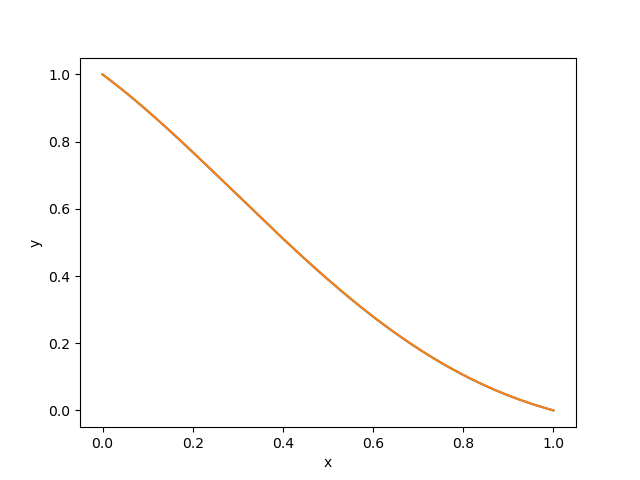
\includegraphics[width=0.9\linewidth]{./pics/final/possion/dgnet1d/exact1.png}  
        \caption{exact solution}  
    \end{subfigure}%  
    \begin{subfigure}{0.5\textwidth}  
        \centering  
        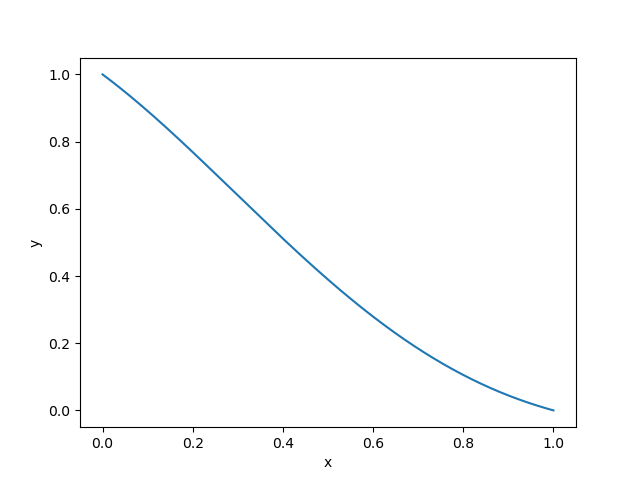
\includegraphics[width=0.9\linewidth]{./pics/final/possion/dgnet1d/pwnn1.png}  
        \caption{Particle WNN}
    \end{subfigure}  

    \begin{subfigure}{0.5\textwidth}  
        \centering  
        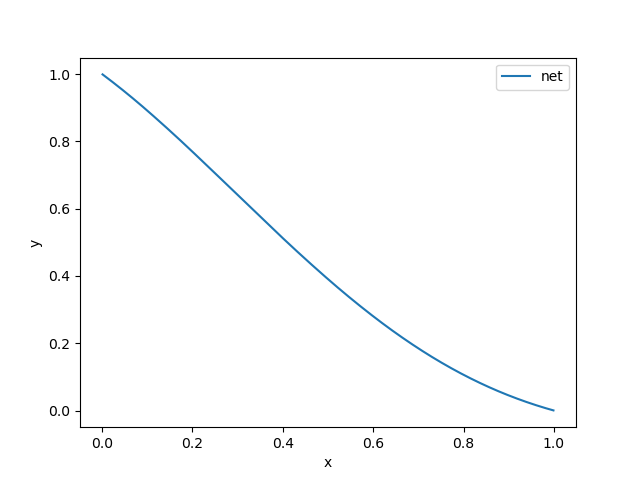
\includegraphics[width=0.9\linewidth]{./pics/final/possion/dgnet1d/splitpwnn1.png}  
        \caption{Split Particle WNN}  
    \end{subfigure}%  
    \begin{subfigure}{0.5\textwidth}  
        \centering  
        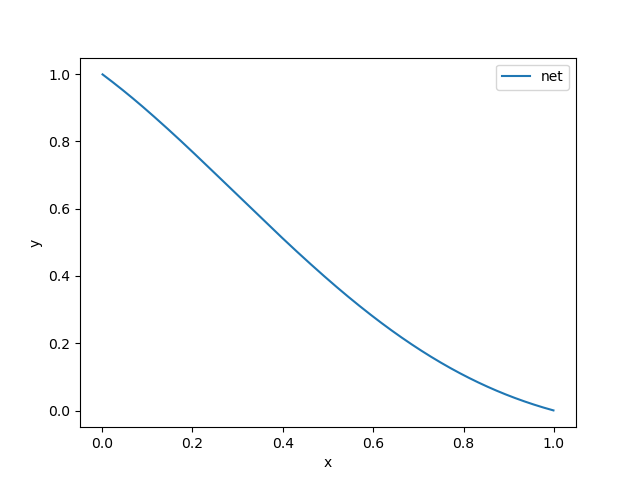
\includegraphics[width=0.9\linewidth]{./pics/final/possion/dgnet1d/dgnet1.png}  
        \caption{Split DG Net}
    \end{subfigure} 
\end{figure} 

\subsection*{$f=10$ with homogeneous DBC}
具有其次边界条件的Possion方程,网络参数和上述相同。
\begin{figure}[H]
    \centering  
    \begin{subfigure}{0.5\textwidth}  
        \centering  
        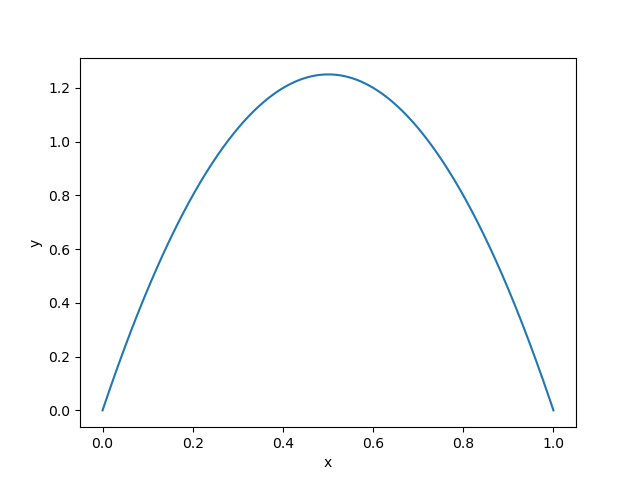
\includegraphics[width=0.9\linewidth]{./pics/final/possion/dgnet1d/pwnn2.png}  
        \caption{Particle WNN}
    \end{subfigure}  

    \begin{subfigure}{0.5\textwidth}  
        \centering  
        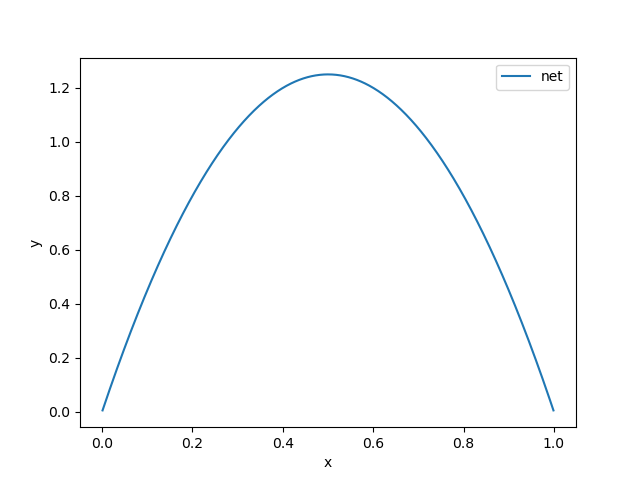
\includegraphics[width=0.9\linewidth]{./pics/final/possion/dgnet1d/splitpwnn2.png}  
        \caption{Split Particle WNN}  
    \end{subfigure}%  
    \begin{subfigure}{0.5\textwidth}  
        \centering  
        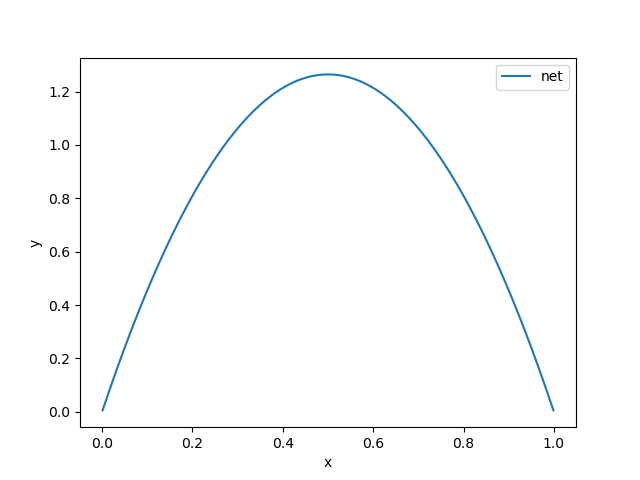
\includegraphics[width=0.9\linewidth]{./pics/final/possion/dgnet1d/dgnet2.png}  
        \caption{Split DG Net}
    \end{subfigure} 
\end{figure} 

\subsection*{$y = xcos(\omega x)$}
当$w=2\pi$时,低频解:

\begin{figure}[H]
    \centering  
    \begin{subfigure}{0.5\textwidth}  
        \centering  
        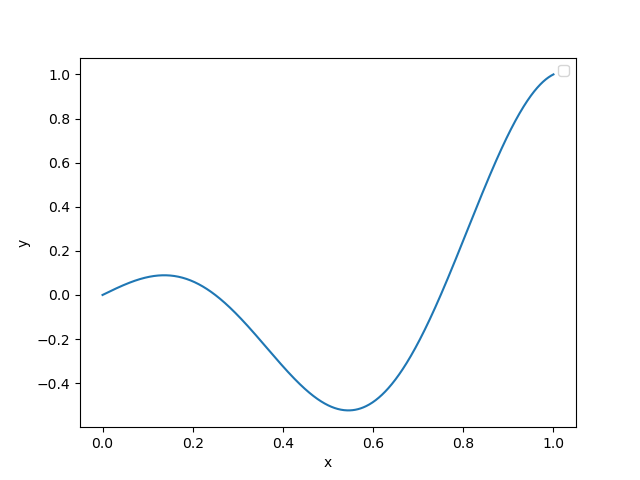
\includegraphics[width=0.9\linewidth]{./pics/final/possion/dgnet1d/2piexact.png}  
        \caption{Exact}  
    \end{subfigure}%  
    \begin{subfigure}{0.5\textwidth}  
        \centering  
        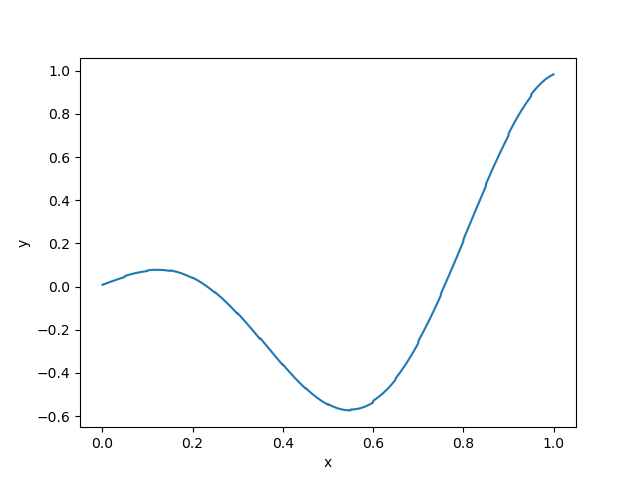
\includegraphics[width=0.9\linewidth]{./pics/final/possion/dgnet1d/2pi2ltrunk.png}  
        \caption{Split DG Net}
    \end{subfigure}  
\end{figure} 

当$w=15\pi$时,高频解:

\begin{figure}[H]
    \centering  
    \begin{subfigure}{0.5\textwidth}  
        \centering  
        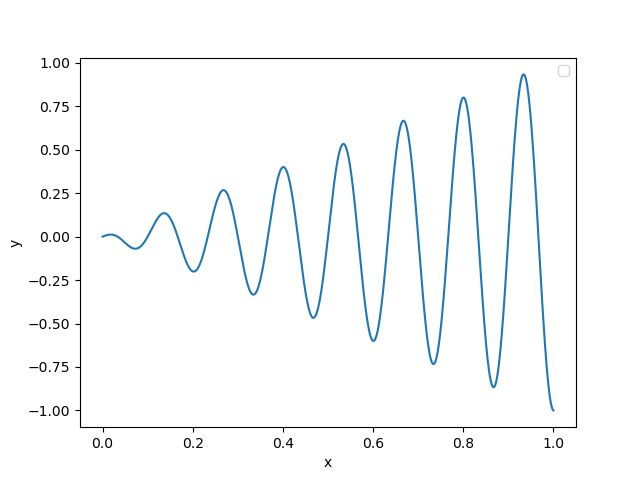
\includegraphics[width=0.9\linewidth]{./pics/final/possion/dgnet1d/15piexact.png}  
        \caption{Exact}  
    \end{subfigure}%  
    \begin{subfigure}{0.5\textwidth}  
        \centering  
        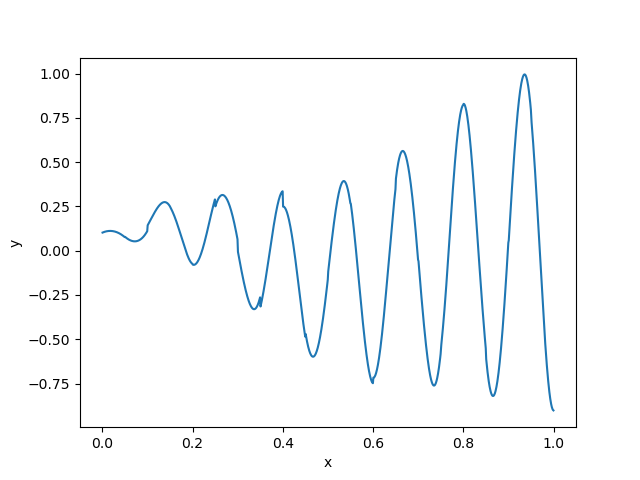
\includegraphics[width=0.9\linewidth]{./pics/final/possion/dgnet1d/15pi2ltrunk.png}  
        \caption{Split DG Net}
    \end{subfigure}  
    \begin{subfigure}{0.45\textwidth}  
        \centering  
        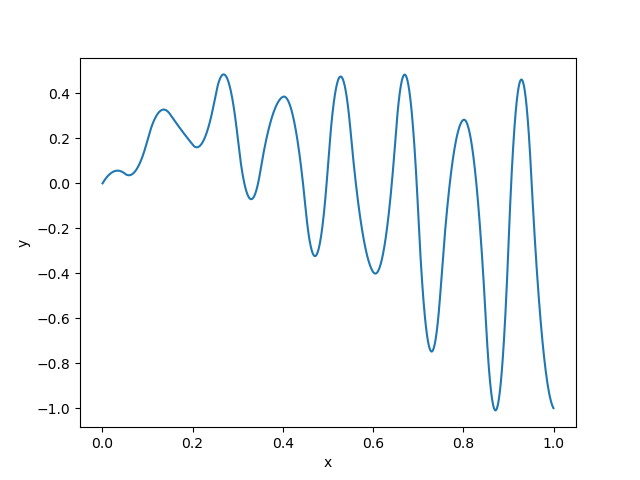
\includegraphics[width=0.9\linewidth]{./pics/final/possion/dgnet1d/15pispwnn.png}  
        \caption{Split PWNN}
    \end{subfigure}  
    \begin{subfigure}{0.5\textwidth}  
        \centering  
        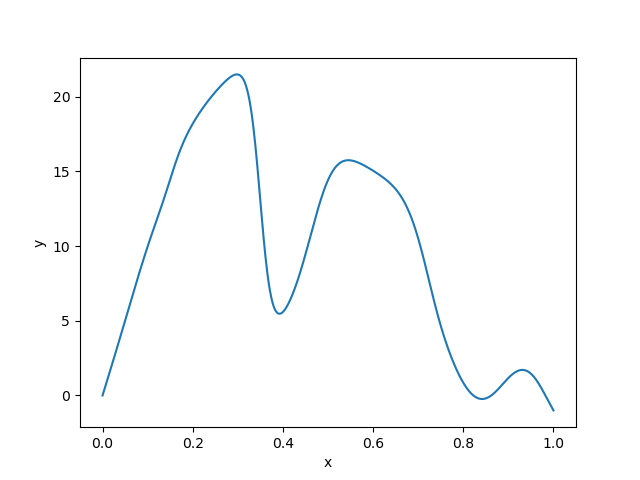
\includegraphics[width=0.9\linewidth]{./pics/final/possion/dgnet1d/15pipwnn.png}  
        \caption{PWNN}
    \end{subfigure} 
\end{figure} 

\section{2D Possion}
\begin{figure}[H]
    \centering  
    \begin{subfigure}{0.45\textwidth}  
        \centering  
        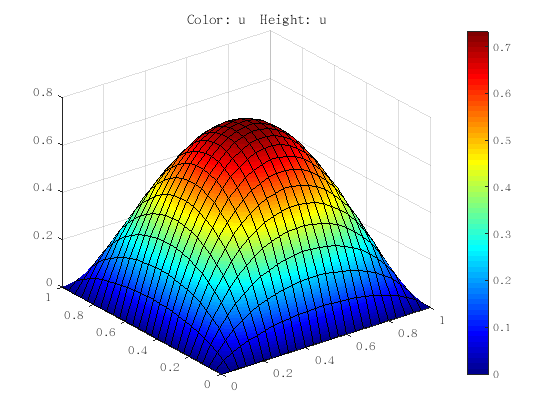
\includegraphics[width=0.9\linewidth]{./pics/final/possion/dgnet2d/exact.png}  
        \caption{Split DG Net}
    \end{subfigure}  
    \begin{subfigure}{0.5\textwidth}  
        \centering  
        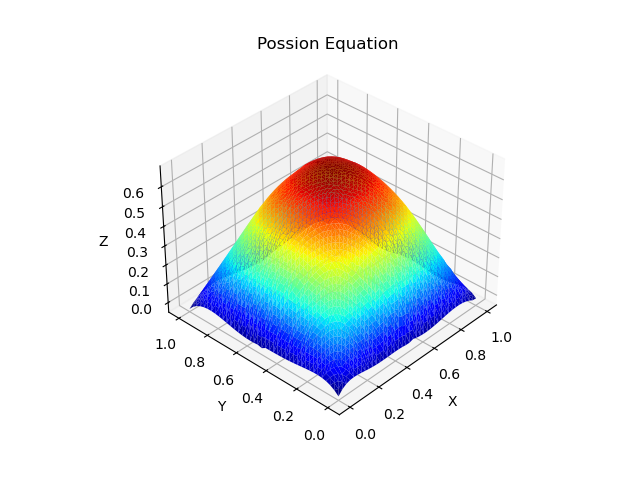
\includegraphics[width=0.9\linewidth]{./pics/final/possion/dgnet2d/dgnetl3gelu3000para0_1.png}  
        \caption{Split DG Net}
    \end{subfigure}  
\end{figure} 

上处图像并非由PWNN官方程序生成,因此无论是训练速度和训练精度可能和官方有些差距。代码还有很大的优化空间。不幸的是因为时间原因,只能到此地步。
